\documentclass[12pt,a4paper]{article}
\usepackage{amsmath, amssymb, geometry, booktabs, xcolor, hyperref,
            listings, pgfplots, tcolorbox, enumitem, fancyhdr, tikz, array}
\usepgfplotslibrary{fillbetween}
\geometry{margin=2.5cm}
\pgfplotsset{compat=1.18}
\tcbuselibrary{skins, breakable}

% Define custom environments
\newtcolorbox{curiositybox}[1]{colback=yellow!10, colframe=orange!80, title=#1, breakable}
\newtcolorbox{infobox}[1]{colback=blue!5, colframe=blue!60, title=#1, breakable}
\newtcolorbox{mistakebox}[1]{colback=red!5, colframe=red!60, title=#1, breakable}
\newtcolorbox{learnbox}[1]{colback=green!5, colframe=green!60, title=#1, breakable}

% Header and Footer
\pagestyle{fancy}
\fancyhf{}
\lhead{Multiple Integrals}
\rhead{Unit 5 --- LAC}
\cfoot{\thepage}

% Document Title Setup
\title{\textbf{Multiple Integrals} \\ \large Unit 5: Multiple Integrals and Coordinate Transformations}
\author{Department of Mathematics}
\date{\today}

\begin{document}
\maketitle
\tableofcontents
\newpage

%=============================================================
\section{Real-World Engineering Hook}
%=============================================================

\begin{curiositybox}{Why Should an Engineer Care?}
Imagine you are designing a composite structural panel for an aircraft wing. The panel is made of two materials bonded together, and the mass density varies continuously across its 2D cross-section according to a known function \(\rho(x,y)\). To calculate the total weight of the panel --- a number that directly determines whether the aircraft can fly safely --- you must integrate \(\rho(x,y)\) over the panel's 2D domain. If you confuse a Type~I region (where you integrate \(y\) first, from curve to curve, then \(x\)) with a Type~II region (where you integrate \(x\) first, from curve to curve, then \(y\)), you set up the wrong limits of integration. The numerical result can be off by a factor of 2 or more, producing a mass estimate that is dangerously incorrect and compromising the aircraft's structural safety margin.

Similarly, in semiconductor device modelling, the net electric charge stored in a 3D volumetric region of doped silicon is \(Q = \iiint_V \rho_e(x,y,z)\,dV\). An incorrect ordering of integration limits for the triple integral yields the wrong charge, leading to flawed transistor design. Multiple integrals are not abstract exercises --- they are the direct computational tool for any physical quantity that accumulates over a 2D or 3D domain.
\end{curiositybox}

%=============================================================
\section{Why This Topic Exists}
%=============================================================

\begin{center}
\begin{tabular}{@{}p{0.40\linewidth} p{0.52\linewidth}@{}}
\toprule
\textbf{Theoretical Concept} & \textbf{Engineering Application / Consequence of Misunderstanding} \\
\midrule
Double integral over a Type~I region \((a \le x \le b,\; g_1(x) \le y \le g_2(x))\) &
  Area, pressure force, and flux computations in structural analysis. A wrong choice of region type reverses the limit dependency and gives an incorrect load calculation on a beam cross-section. \\[4pt]
Double integral over a Type~II region \((c \le y \le d,\; h_1(y) \le x \le h_2(y))\) &
  Used when the natural bounding curves are expressed as functions of \(y\). Choosing the wrong region type forces non-existent functions of \(x\), making the integral impossible to set up correctly. \\[4pt]
Change of order of integration &
  Simplifies analytically intractable integrals in heat transfer (\(\int e^{y^2}\,dy\) has no closed form) and fluid mechanics. Failing to reverse \emph{both} limits and the integration variable order gives a completely different (wrong) integral. \\[4pt]
Triple integrals &
  Volume, mass, centre of mass, and moment of inertia of 3D solid components in mechanical and civil engineering. An error in the innermost limit's dependence on outer variables propagates through every layer of integration. \\
\bottomrule
\end{tabular}
\end{center}

\begin{learnbox}{Core Learning Objective}
By the end of this topic you will be able to: (i) identify whether a 2D region is Type~I or Type~II, (ii) set up and evaluate double integrals in both orders using Fubini's theorem, (iii) change the order of integration when the original order is analytically intractable, and (iv) extend all these ideas to triple integrals over 3D regions with variable limits.
\end{learnbox}

%=============================================================
\section{Intuition First \& Mathematical Definitions}
%=============================================================

\subsection{Double Integrals over Type I and Type II Regions}

Think of integrating a function \(f(x,y)\) over a 2D region \(R\) as stacking infinitely many thin strips. If the strips are \emph{vertical} --- each strip runs from a lower curve to an upper curve for a fixed \(x\) --- the region is \textbf{Type~I}. If the strips are \emph{horizontal} --- each strip runs from a left curve to a right curve for a fixed \(y\) --- the region is \textbf{Type~II}. Fubini's theorem tells us we can compute the double integral as two successive ordinary (single-variable) integrals in either order, provided the integrand is continuous on the region.

\begin{infobox}{Double Integrals: Type I and Type II Regions}
\textbf{Type I Region.} A region \(R\) in the \(xy\)-plane is of \emph{Type I} if
\[
  R = \{(x,y) \mid a \le x \le b,\; g_1(x) \le y \le g_2(x)\}
\]
where \(g_1\) and \(g_2\) are continuous on \([a,b]\) and \(g_1(x) \le g_2(x)\).

\textbf{Type II Region.} A region \(R\) is of \emph{Type II} if
\[
  R = \{(x,y) \mid c \le y \le d,\; h_1(y) \le x \le h_2(y)\}
\]
where \(h_1\) and \(h_2\) are continuous on \([c,d]\) and \(h_1(y) \le h_2(y)\).

\textbf{Fubini's Theorem (Double Integral).} If \(f\) is continuous on \(R\), then:

\emph{Over a Type I region:}
\[
  \iint_R f(x,y)\,dA = \int_a^b \int_{g_1(x)}^{g_2(x)} f(x,y)\,dy\,dx
\]

\emph{Over a Type II region:}
\[
  \iint_R f(x,y)\,dA = \int_c^d \int_{h_1(y)}^{h_2(y)} f(x,y)\,dx\,dy
\]

\textbf{Key Properties.}
\begin{itemize}[nosep]
  \item Linearity: \(\iint_R [af+bg]\,dA = a\iint_R f\,dA + b\iint_R g\,dA\).
  \item If \(R = R_1 \cup R_2\) with \(R_1 \cap R_2\) having zero area, then \(\iint_R f\,dA = \iint_{R_1} f\,dA + \iint_{R_2} f\,dA\).
  \item The area of \(R\) is \(\iint_R 1\,dA\).
\end{itemize}
\end{infobox}

\textbf{Worked Example 3.1 --- Type I Region.}
Evaluate \(\displaystyle\iint_R (x + 2y)\,dA\) where \(R\) is the triangular region with vertices \((0,0)\), \((2,0)\), and \((2,4)\).

\textit{Step 1: Identify the region.} The boundary edges are: \(x=0\) (left, but the left vertex is at origin; however the triangle has vertices \((0,0)\), \((2,0)\), \((2,4)\)), so the edges are the segment from \((0,0)\) to \((2,0)\) along \(y=0\), the segment from \((2,0)\) to \((2,4)\) along \(x=2\), and the hypotenuse from \((0,0)\) to \((2,4)\) with slope \(4/2=2\), i.e.\ \(y=2x\).

\textit{Step 2: Express as a Type I region.} For \(0 \le x \le 2\), \(y\) runs from \(y=0\) (bottom) to \(y=2x\) (hypotenuse). So
\[
  R:\quad 0 \le x \le 2,\quad 0 \le y \le 2x.
\]

\textit{Step 3: Inner integral} (integrate over \(y\)):
\[
  \int_0^{2x}(x+2y)\,dy = \left[xy + y^2\right]_0^{2x} = x(2x) + (2x)^2 = 2x^2 + 4x^2 = 6x^2.
\]

\textit{Step 4: Outer integral} (integrate over \(x\)):
\[
  \int_0^2 6x^2\,dx = \left[2x^3\right]_0^2 = 2(8) - 0 = 16.
\]

\textbf{Answer:} \(\displaystyle\iint_R (x+2y)\,dA = 16\).

\vspace{4pt}
\textbf{Worked Example 3.2 --- Type II Region.}
Evaluate \(\displaystyle\iint_R 3y\,dA\) where \(R\) is the region bounded by \(x = y^2\) and \(x = y + 2\) (a Type II region).

\textit{Step 1: Find intersection.} \(y^2 = y+2 \Rightarrow y^2-y-2=0 \Rightarrow (y-2)(y+1)=0\). So \(y = -1\) and \(y = 2\).

\textit{Step 2: Type II description.} For \(-1 \le y \le 2\), \(x\) runs from \(x = y^2\) (left) to \(x = y+2\) (right):
\[
  R:\quad -1 \le y \le 2,\quad y^2 \le x \le y+2.
\]

\textit{Step 3: Inner integral}:
\[
  \int_{y^2}^{y+2} 3y\,dx = 3y\bigl[(y+2)-y^2\bigr] = 3y(y+2-y^2) = 3y^2 + 6y - 3y^3.
\]

\textit{Step 4: Outer integral}:
\[
  \int_{-1}^{2}(3y^2+6y-3y^3)\,dy = \left[y^3 + 3y^2 - \tfrac{3}{4}y^4\right]_{-1}^{2}.
\]
At \(y=2\): \(8 + 12 - 12 = 8\). At \(y=-1\): \(-1+3 - \tfrac{3}{4} = 2 - \tfrac{3}{4} = \tfrac{5}{4}\).

Result: \(8 - \tfrac{5}{4} = \tfrac{27}{4}\).

\textbf{Answer:} \(\displaystyle\iint_R 3y\,dA = \dfrac{27}{4}\).

%---------------------------------------------------------------
\subsection{Change of Order of Integration}

Some double integrals are set up in an order that makes the \emph{inner} integral impossible to evaluate analytically --- for instance, integrating \(e^{y^2}\) with respect to \(y\) has no elementary antiderivative. In such cases, we \textbf{change the order of integration}: we re-sketch the region, re-read the same region in the opposite order (swapping the roles of inner and outer variables), and often obtain an integral that is immediately tractable. The key insight is that the \emph{geometric region} does not change --- only the way we slice it changes.

\begin{infobox}{Change of Order of Integration}
\textbf{When to apply.} Change the order when the inner integral \(\int f(x,y)\,dy\) (or \(\int f(x,y)\,dx\)) has no closed-form antiderivative in the current variable, or when the integrand simplifies dramatically in the other order.

\textbf{Procedure.}
\begin{enumerate}[nosep]
  \item \textbf{Sketch the region} \(R\) defined by the original limits.
  \item \textbf{Re-describe \(R\)} in the reversed order: find the constant outer limits and the variable inner limits in the new arrangement.
  \item \textbf{Rewrite the integral} with new limits. Do not change the integrand \(f(x,y)\) itself; only the limits and the order of \(dx\,dy\) change.
  \item \textbf{Evaluate} the new (hopefully simpler) integral.
\end{enumerate}

\textbf{Caution.} When reversing order, both sets of limits change. A common error is to swap only the differential symbols \(dx\,dy \to dy\,dx\) while keeping the original numerical limits --- this gives an entirely incorrect integral.

\textbf{Formula (conceptual).}
\[
  \int_a^b \int_{g_1(x)}^{g_2(x)} f(x,y)\,dy\,dx
  \;=\;
  \int_c^d \int_{h_1(y)}^{h_2(y)} f(x,y)\,dx\,dy
\]
where the right-hand side describes the \emph{same geometric region} \(R\) as a Type II region.
\end{infobox}

\textbf{Worked Example 3.3 --- Change of Order.}
Evaluate \(\displaystyle I = \int_0^1 \int_x^1 e^{y^2}\,dy\,dx\).

\textit{Step 1: Attempt original order.} The inner integral is \(\int_x^1 e^{y^2}\,dy\). The function \(e^{y^2}\) has no elementary antiderivative; this order is analytically intractable.

\textit{Step 2: Sketch and re-describe the region.}
Original limits: \(0 \le x \le 1\) (outer), \(x \le y \le 1\) (inner). This describes the triangle \(R\) with corners \((0,0)\), \((0,1)\), \((1,1)\) --- the region where \(0 \le x \le y\) and \(0 \le y \le 1\).

Re-describe as Type II: fix \(y\) from \(0\) to \(1\); for each \(y\), \(x\) runs from \(0\) to \(y\).
\[
  R:\quad 0 \le y \le 1,\quad 0 \le x \le y.
\]

\textit{Step 3: Rewrite integral.}
\[
  I = \int_0^1 \int_0^y e^{y^2}\,dx\,dy.
\]

\textit{Step 4: Inner integral} (integrate over \(x\), treating \(y\) as constant):
\[
  \int_0^y e^{y^2}\,dx = e^{y^2}\bigl[x\bigr]_0^y = y\,e^{y^2}.
\]

\textit{Step 5: Outer integral}:
\[
  I = \int_0^1 y\,e^{y^2}\,dy.
\]
Let \(u = y^2\), so \(du = 2y\,dy\), i.e.\ \(y\,dy = \tfrac{1}{2}du\). When \(y=0\), \(u=0\); when \(y=1\), \(u=1\).
\[
  I = \int_0^1 e^u \cdot \tfrac{1}{2}\,du = \tfrac{1}{2}\bigl[e^u\bigr]_0^1 = \tfrac{1}{2}(e^1 - e^0) = \tfrac{e-1}{2}.
\]

\textbf{Answer:} \(\displaystyle I = \dfrac{e-1}{2} \approx 0.8591\).

%---------------------------------------------------------------
\subsection{Triple Integrals}

Just as a double integral sums a function over a 2D region, a \textbf{triple integral} sums a function over a 3D solid region \(V\). Physically, if \(f(x,y,z)\) is a density (mass per unit volume), the triple integral gives total mass; if \(f=1\), it gives the volume of \(V\). The key challenge is correctly establishing the limits: the \emph{innermost} limits may depend on the two outer variables, the \emph{middle} limits may depend on the outermost variable, and only the \emph{outermost} limits are constants.

\begin{infobox}{Triple Integrals}
\textbf{Definition.} Let \(f(x,y,z)\) be continuous on a bounded solid region \(V \subset \mathbb{R}^3\). The triple integral is
\[
  \iiint_V f(x,y,z)\,dV = \lim_{l,m,n\to\infty}\sum_{i=1}^{l}\sum_{j=1}^{m}\sum_{k=1}^{n} f(x_{ijk}^*, y_{ijk}^*, z_{ijk}^*)\,\Delta V_{ijk}.
\]

\textbf{Fubini's Theorem (Triple Integral).} If \(f\) is continuous on
\[
  V = \{(x,y,z)\mid a\le x\le b,\; g_1(x)\le y\le g_2(x),\; \phi_1(x,y)\le z\le \phi_2(x,y)\},
\]
then
\[
  \iiint_V f\,dV = \int_a^b \int_{g_1(x)}^{g_2(x)} \int_{\phi_1(x,y)}^{\phi_2(x,y)} f(x,y,z)\,dz\,dy\,dx.
\]

\textbf{Six Possible Iteration Orders} (all equal for continuous \(f\) on nice regions):
\[
  dz\,dy\,dx,\quad dz\,dx\,dy,\quad dy\,dz\,dx,\quad dy\,dx\,dz,\quad dx\,dz\,dy,\quad dx\,dy\,dz.
\]

\textbf{Special cases.}
\begin{itemize}[nosep]
  \item Volume: \(\iiint_V 1\,dV = \text{Vol}(V)\).
  \item Mass: \(M = \iiint_V \rho(x,y,z)\,dV\) where \(\rho\) is mass density.
  \item Over a rectangular box \([a,b]\times[c,d]\times[p,q]\):
    \(\iiint_V f\,dV = \int_a^b\int_c^d\int_p^q f\,dz\,dy\,dx\) (limits are all constants).
\end{itemize}
\end{infobox}

\textbf{Worked Example 3.4 --- Triple Integral over a Rectangular Box.}
Evaluate \(\displaystyle\iiint_V (x + yz)\,dV\) where \(V = [0,1]\times[0,2]\times[0,3]\).

\textit{Step 1: Inner integral} (over \(z\), \(0\le z\le 3\)):
\[
  \int_0^3 (x+yz)\,dz = \left[xz + \tfrac{1}{2}yz^2\right]_0^3 = 3x + \tfrac{9}{2}y.
\]

\textit{Step 2: Middle integral} (over \(y\), \(0\le y\le 2\)):
\[
  \int_0^2 \left(3x + \tfrac{9}{2}y\right)dy = \left[3xy + \tfrac{9}{4}y^2\right]_0^2 = 6x + 9.
\]

\textit{Step 3: Outer integral} (over \(x\), \(0\le x\le 1\)):
\[
  \int_0^1 (6x+9)\,dx = \left[3x^2 + 9x\right]_0^1 = 3 + 9 = 12.
\]

\textbf{Answer:} \(\displaystyle\iiint_V (x+yz)\,dV = 12\).

\vspace{4pt}
\textbf{Worked Example 3.5 --- Triple Integral over a Non-Rectangular Region.}
Evaluate \(\displaystyle\iiint_V x\,dV\) where \(V = \{0 \le x \le 1,\; 0 \le y \le x,\; 0 \le z \le x+y\}\).

\textit{Step 1: Inner integral} (over \(z\), \(0 \le z \le x+y\)):
\[
  \int_0^{x+y} x\,dz = x(x+y) = x^2 + xy.
\]

\textit{Step 2: Middle integral} (over \(y\), \(0 \le y \le x\)):
\[
  \int_0^{x}(x^2+xy)\,dy = \left[x^2 y + \tfrac{1}{2}xy^2\right]_0^x = x^3 + \tfrac{1}{2}x^3 = \tfrac{3}{2}x^3.
\]

\textit{Step 3: Outer integral} (over \(x\), \(0 \le x \le 1\)):
\[
  \int_0^1 \tfrac{3}{2}x^3\,dx = \tfrac{3}{2}\cdot\left[\tfrac{x^4}{4}\right]_0^1 = \tfrac{3}{8}.
\]

\textbf{Answer:} \(\displaystyle\iiint_V x\,dV = \dfrac{3}{8}\).

%=============================================================
\section{Visual Artifacts \& Geometric Interpretation}
%=============================================================

\subsection*{Figure 1: Type I Region --- Vertical Strips}

\begin{center}
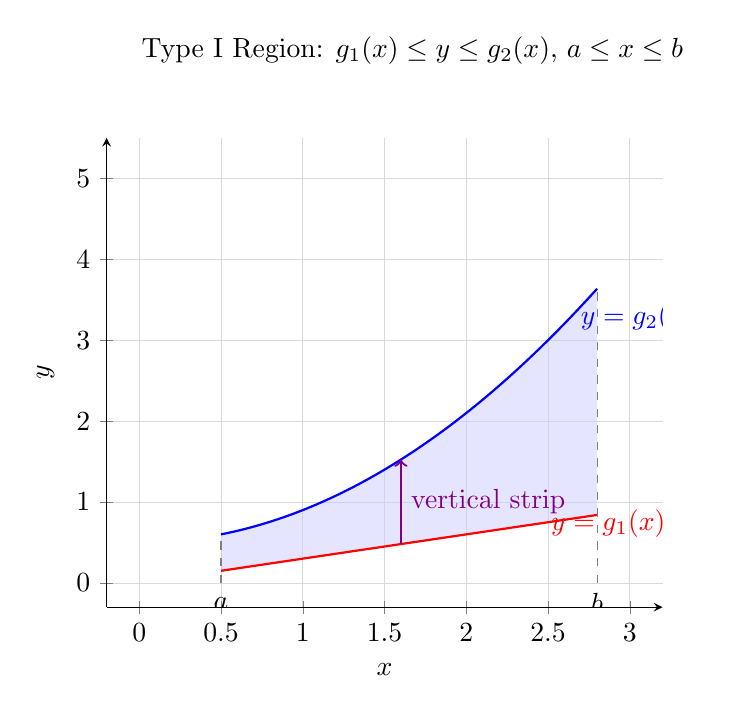
\begin{tikzpicture}[scale=1.1]
  \begin{axis}[
    xlabel={$x$}, ylabel={$y$},
    xmin=-0.2, xmax=3.2,
    ymin=-0.3, ymax=5.5,
    axis lines=left,
    grid=both,
    grid style={line width=0.3pt, draw=gray!30},
    width=8cm, height=7cm,
    title={Type I Region: $g_1(x)\le y\le g_2(x)$, $a\le x\le b$}
  ]
    \addplot[name path=upper, thick, blue, domain=0.5:2.8, samples=60]
      {0.4*x^2 + 0.5} node[right, pos=0.9]{$y=g_2(x)$};
    \addplot[name path=lower, thick, red, domain=0.5:2.8, samples=60]
      {0.3*x} node[right, pos=0.85]{$y=g_1(x)$};
    \addplot[blue!20, opacity=0.5] fill between[of=upper and lower,
      soft clip={domain=0.5:2.8}];
    \draw[dashed, gray] (axis cs:0.5,0) -- (axis cs:0.5,{0.4*0.5^2+0.5});
    \draw[dashed, gray] (axis cs:2.8,0) -- (axis cs:2.8,{0.4*2.8^2+0.5});
    \node at (axis cs:0.5,-0.25) {$a$};
    \node at (axis cs:2.8,-0.25) {$b$};
    \draw[->, thick, violet] (axis cs:1.6, {0.3*1.6}) -- (axis cs:1.6, {0.4*1.6^2+0.5})
      node[midway, right]{vertical strip};
  \end{axis}
\end{tikzpicture}
\end{center}

\subsection*{Figure 2: Type II Region --- Horizontal Strips}

\begin{center}
\begin{tikzpicture}[scale=1.1]
  \begin{axis}[
    xlabel={$x$}, ylabel={$y$},
    xmin=-0.2, xmax=5.5,
    ymin=-0.2, ymax=3.2,
    axis lines=left,
    grid=both,
    grid style={line width=0.3pt, draw=gray!30},
    width=8cm, height=7cm,
    title={Type II Region: $h_1(y)\le x\le h_2(y)$, $c\le y\le d$}
  ]
    \addplot[name path=right, thick, blue, domain=0.4:2.8, samples=60]
      ({0.5*x^2+0.3}, x) node[above, pos=0.9]{$x=h_2(y)$};
    \addplot[name path=left2, thick, red, domain=0.4:2.8, samples=60]
      ({0.4*x}, x) node[above left, pos=0.85]{$x=h_1(y)$};
    \addplot[blue!20, opacity=0.5] fill between[of=right and left2,
      soft clip={domain=0.4:2.8}];
    \draw[dashed, gray] (0,axis cs:0,0.4) -- ({0.4*0.4},axis cs:0,0.4);
    \node at (axis cs:-0.25, 0.4) {$c$};
    \node at (axis cs:-0.25, 2.8) {$d$};
    \draw[->, thick, violet] (axis cs:{0.4*1.6},1.6) -- (axis cs:{0.5*1.6^2+0.3},1.6)
      node[midway, above]{horiz.\ strip};
  \end{axis}
\end{tikzpicture}
\end{center}

\subsection*{Figure 3: Volume Under a Surface \(z = f(x,y)\) Over a 2D Region}

\begin{center}
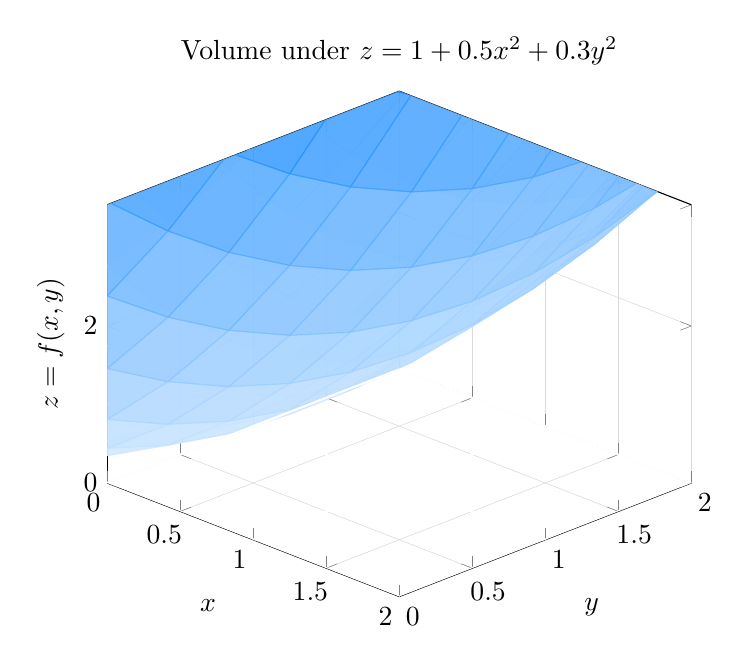
\begin{tikzpicture}
  \begin{axis}[
    xlabel={$x$}, ylabel={$y$}, zlabel={$z=f(x,y)$},
    xmin=0, xmax=2, ymin=0, ymax=2, zmin=0,
    grid=both,
    grid style={line width=0.2pt, draw=gray!30},
    view={45}{30},
    colormap/cool,
    width=9cm, height=8cm,
    title={Volume under $z = 1 + 0.5x^2 + 0.3y^2$},
    samples=25
  ]
    \addplot3[surf, opacity=0.75, shader=flat]
      {1 + 0.5*x^2 + 0.3*y^2};
    \addplot3[domain=0:2, domain y=0:2, samples=3, samples y=3,
      thick, black, mesh] {0};
  \end{axis}
\end{tikzpicture}
\end{center}

The volume of the solid lying between the \(xy\)-plane and the surface \(z=f(x,y)\) over the region \(R\) is exactly \(\iint_R f(x,y)\,dA\).

%=============================================================
\section{Step-by-Step Algorithmic Workflow}
%=============================================================

\begin{center}
\fbox{
\begin{minipage}{0.88\linewidth}
\textbf{Algorithmic Workflow for Multiple Integrals}

\begin{enumerate}
  \item \textbf{Sketch the region.} Draw the boundary curves or surfaces. Label all intersection points. Shade the interior of \(R\) (or \(V\)).

  \item \textbf{Identify region type (2D).}
    \begin{itemize}[nosep]
      \item Can you describe the boundary as upper/lower functions of \(x\)? \(\Rightarrow\) \textbf{Type I}.
      \item Can you describe the boundary as right/left functions of \(y\)? \(\Rightarrow\) \textbf{Type II}.
      \item If both, prefer the order that gives simpler limit expressions.
    \end{itemize}

  \item \textbf{Set up limits (double integral).}
    \begin{itemize}[nosep]
      \item Type I: outer limits are constants \(a \le x \le b\); inner limits are \(g_1(x) \le y \le g_2(x)\).
      \item Type II: outer limits are constants \(c \le y \le d\); inner limits are \(h_1(y) \le x \le h_2(y)\).
    \end{itemize}

  \item \textbf{Decision: change order?} If the inner integral \(\int f\,dy\) (or \(\int f\,dx\)) has no closed-form antiderivative, re-sketch the region as the opposite type and rewrite limits. Then proceed.

  \item \textbf{Evaluate inner integral.} Treat the outer variable(s) as constants. Apply standard integration techniques. Simplify the result as a function of the outer variable(s).

  \item \textbf{Evaluate outer integral(s).} For a double integral, integrate the result from Step 5 over the outer constant limits. For a triple integral, repeat Steps 4--5 for two more layers, always working from innermost to outermost.

  \item \textbf{Extend to triple integrals.} Fix the outermost variable \(x \in [a,b]\). For each \(x\), fix the middle variable \(y \in [g_1(x), g_2(x)]\). For each \((x,y)\) pair, integrate over \(z \in [\phi_1(x,y), \phi_2(x,y)]\) --- the innermost limits are functions of \emph{both} outer variables.

  \item \textbf{Check units and sign.} For area/volume integrands, the result must be positive. For signed quantities (net flux, net charge), negative results are physically meaningful.
\end{enumerate}
\end{minipage}
}
\end{center}

%=============================================================
\section{Fully Worked Step-by-Step Numerical Examples}
%=============================================================

\subsection*{Example 1 --- Basic Double Integral over a Triangular Region (Type I)}

Evaluate \(\displaystyle\iint_R xy\,dA\) where \(R\) is the triangular region with vertices \((0,0)\), \((3,0)\), and \((3,3)\).

\textit{Step 1: Identify region.} The hypotenuse connects \((0,0)\) and \((3,3)\), giving the line \(y=x\). For fixed \(x \in [0,3]\), \(y\) runs from \(0\) to \(x\). This is a Type I region:
\[
  R:\quad 0 \le x \le 3,\quad 0 \le y \le x.
\]

\textit{Step 2: Set up integral.}
\[
  I = \int_0^3 \int_0^x xy\,dy\,dx.
\]

\textit{Step 3: Inner integral} (over \(y\)):
\[
  \int_0^x xy\,dy = x\left[\frac{y^2}{2}\right]_0^x = x \cdot \frac{x^2}{2} = \frac{x^3}{2}.
\]

\textit{Step 4: Outer integral} (over \(x\)):
\[
  I = \int_0^3 \frac{x^3}{2}\,dx = \frac{1}{2}\left[\frac{x^4}{4}\right]_0^3 = \frac{1}{2}\cdot\frac{81}{4} = \frac{81}{8}.
\]

\textbf{Answer:} \(\displaystyle\iint_R xy\,dA = \dfrac{81}{8} = 10.125\).

\begin{learnbox}{Key Insight --- Example 1}
For a Type I region, read the inner integral limits directly from the bounding curves expressed as functions of \(x\). Here, \(y\) runs from the \(x\)-axis (\(y=0\)) up to the hypotenuse (\(y=x\)).
\end{learnbox}

\subsection*{Example 2 --- Change of Order of Integration}

Evaluate \(\displaystyle I = \int_0^1 \int_x^1 e^{y^2}\,dy\,dx\).

\textit{Step 1: Observe that the inner integral} \(\int_x^1 e^{y^2}\,dy\) has no elementary antiderivative in \(y\). We must change order.

\textit{Step 2: Describe the region from the original limits.}
Outer: \(0 \le x \le 1\). Inner: \(x \le y \le 1\).
Sketch: this is the triangle with corners \((0,0)\), \((0,1)\), \((1,1)\), where \(y \ge x\) and both lie in \([0,1]\).

\textit{Step 3: Re-describe as Type II.}
For fixed \(y \in [0,1]\), \(x\) ranges from \(0\) to \(y\):
\[
  R:\quad 0 \le y \le 1,\quad 0 \le x \le y.
\]

\textit{Step 4: Rewrite integral.}
\[
  I = \int_0^1 \int_0^y e^{y^2}\,dx\,dy.
\]

\textit{Step 5: Inner integral} (over \(x\), holding \(y\) constant):
\[
  \int_0^y e^{y^2}\,dx = e^{y^2}\cdot y.
\]

\textit{Step 6: Outer integral} (substitution \(u=y^2\), \(du=2y\,dy\)):
\[
  I = \int_0^1 ye^{y^2}\,dy = \frac{1}{2}\int_0^1 e^u\,du = \frac{1}{2}\bigl[e^u\bigr]_0^1 = \frac{e-1}{2}.
\]

\textbf{Answer:} \(\displaystyle I = \dfrac{e-1}{2} \approx 0.8591\).

\begin{learnbox}{Key Insight --- Example 2}
When the inner integral is intractable (e.g., involves \(e^{y^2}\), \(\sin(x^2)\), \(\cos(y^3)\)), changing the order of integration converts an impossible computation into a straightforward one. Always re-sketch the full geometric region before reversing limits.
\end{learnbox}

\subsection*{Example 3 --- Triple Integral: Mass of a Solid Region}

Compute the mass of the solid \(V = \{0 \le x \le 1,\; 0 \le y \le 1-x,\; 0 \le z \le 1-x-y\}\) with constant density \(\rho(x,y,z) = 6\) kg/m\(^3\).

\textit{Step 1: Set up.} Mass \(= \iiint_V \rho\,dV = \iiint_V 6\,dV\). The region is a tetrahedron with vertices at \((0,0,0)\), \((1,0,0)\), \((0,1,0)\), and \((0,0,1)\).
\[
  M = \int_0^1 \int_0^{1-x} \int_0^{1-x-y} 6\,dz\,dy\,dx.
\]

\textit{Step 2: Inner integral} (over \(z\)):
\[
  \int_0^{1-x-y} 6\,dz = 6(1-x-y).
\]

\textit{Step 3: Middle integral} (over \(y\), \(0 \le y \le 1-x\)):
\[
  \int_0^{1-x} 6(1-x-y)\,dy.
\]
Let \(c = 1-x\) (constant w.r.t.\ \(y\)):
\[
  6\int_0^{c}(c-y)\,dy = 6\left[cy - \frac{y^2}{2}\right]_0^c = 6\left(c^2 - \frac{c^2}{2}\right) = 6\cdot\frac{c^2}{2} = 3c^2 = 3(1-x)^2.
\]

\textit{Step 4: Outer integral} (over \(x\)):
\[
  M = \int_0^1 3(1-x)^2\,dx.
\]
Let \(u = 1-x\), \(du = -dx\); limits: \(x=0\Rightarrow u=1\), \(x=1\Rightarrow u=0\):
\[
  M = 3\int_1^0 u^2(-du) = 3\int_0^1 u^2\,du = 3\cdot\frac{1}{3} = 1.
\]

\textbf{Answer:} The mass of the tetrahedron is \(M = 1\) kg (with density \(6\) kg/m\(^3\) and volume \(\frac{1}{6}\) m\(^3\), giving \(6 \times \frac{1}{6} = 1\) kg, which is consistent).

\textit{Physical interpretation.} A homogeneous tetrahedron occupying the unit simplex (volume \(= 1/6\)) with density \(6\) kg/m\(^3\) has total mass exactly \(1\) kg.

\begin{learnbox}{Key Insight --- Example 3}
For a triple integral over a tetrahedron, the innermost limit \(z = 1-x-y\) depends on \emph{both} outer variables. The middle limit \(y = 1-x\) depends on only the outermost variable. The outermost limit \(x \in [0,1]\) is constant. This dependency chain is the hallmark of non-rectangular 3D regions.
\end{learnbox}

%=============================================================
\section{Tabular Comparison / Workflow Reference}
%=============================================================

\begin{center}
\begin{tabular}{@{}p{0.22\linewidth} p{0.24\linewidth} p{0.24\linewidth} p{0.24\linewidth}@{}}
\toprule
\textbf{Feature} & \textbf{Type I Region} & \textbf{Type II Region} & \textbf{When to choose} \\
\midrule
Outer variable & \(x\) (constant limits \(a,b\)) & \(y\) (constant limits \(c,d\)) & Whichever has constant outer limits \\[3pt]
Inner limits & Functions of \(x\): \(g_1(x) \le y \le g_2(x)\) & Functions of \(y\): \(h_1(y) \le x \le h_2(y)\) & Whichever boundary curves are simpler to express \\[3pt]
Strip direction & Vertical & Horizontal & Determined by how boundaries are given \\[3pt]
Preferred integrand form & \(f(x,y)\) easily integrated in \(y\) first & \(f(x,y)\) easily integrated in \(x\) first & Choose order making inner integral tractable \\[3pt]
Example region & \(0\le x\le 2\), \(0\le y\le x^2\) & \(0\le y\le 4\), \(0\le x\le \sqrt{y}\) & Both describe the same parabolic region \\
\bottomrule
\end{tabular}
\end{center}

\vspace{10pt}

\begin{center}
\begin{tabular}{@{}p{0.15\linewidth} p{0.45\linewidth} p{0.34\linewidth}@{}}
\toprule
\textbf{Order} & \textbf{Limit Structure} & \textbf{Best when \ldots} \\
\midrule
\(dz\,dy\,dx\) & \(\int_a^b\int_{g_1(x)}^{g_2(x)}\int_{\phi_1(x,y)}^{\phi_2(x,y)}\,dz\,dy\,dx\) & Projection onto \(xy\)-plane is simplest \\[3pt]
\(dz\,dx\,dy\) & \(\int_c^d\int_{h_1(y)}^{h_2(y)}\int_{\phi_1(x,y)}^{\phi_2(x,y)}\,dz\,dx\,dy\) & Projection onto \(xy\)-plane, \(y\) outer \\[3pt]
\(dy\,dz\,dx\) & \(\int_a^b\int_{p(x)}^{q(x)}\int_{u(x,z)}^{v(x,z)}\,dy\,dz\,dx\) & Projection onto \(xz\)-plane is simplest \\[3pt]
\(dy\,dx\,dz\) & \(\int_p^q\int_{r(z)}^{s(z)}\int_{u(x,z)}^{v(x,z)}\,dy\,dx\,dz\) & \(z\) is the natural outermost variable \\[3pt]
\(dx\,dz\,dy\) & \(\int_c^d\int_{p(y)}^{q(y)}\int_{u(y,z)}^{v(y,z)}\,dx\,dz\,dy\) & Projection onto \(yz\)-plane, \(y\) outer \\[3pt]
\(dx\,dy\,dz\) & \(\int_p^q\int_{c(z)}^{d(z)}\int_{u(y,z)}^{v(y,z)}\,dx\,dy\,dz\) & Projection onto \(yz\)-plane is simplest \\
\bottomrule
\end{tabular}
\end{center}

%=============================================================
\section{Common Student Mistakes \& Pitfalls}
%=============================================================

\begin{mistakebox}{Common Mistakes in Multiple Integrals}
\begin{tabular}{@{}>{\raggedright}p{0.30\linewidth} >{\raggedright}p{0.30\linewidth} >{\raggedright\arraybackslash}p{0.32\linewidth}@{}}
\toprule
\textbf{Mistake Made} & \textbf{Why Students Do It} & \textbf{Correct Mathematical Approach} \\
\midrule
Using Type I limits \((a\le x\le b, g_1(x)\le y\le g_2(x))\) when the region should be Type II &
  The student writes limits in the order they first see the boundary curves, without sketching the region &
  Always sketch the region first. If boundary curves are naturally expressed as \(x=h(y)\), use Type II limits and integrate \(x\) in the inner integral \\[6pt]
Keeping original numerical limits when changing order of integration (e.g., swapping \(dx\,dy\) to \(dy\,dx\) but keeping the same numbers) &
  Students treat the variable swap as purely symbolic, forgetting that the limits are functions of the integration variables &
  Re-read the region geometrically after the swap. Re-derive both the inner and outer limits from scratch by sketching and identifying bounding curves in the new order \\[6pt]
Setting up triple integral limits as all constants (treating every variable as independent) when the region is not a rectangular box &
  Students copy the rectangular-box formula without checking whether inner limits depend on outer variables &
  Identify the dependency chain: innermost limits may depend on both middle and outer variables; middle limits may depend on only the outer variable. Establish limits by fixing outer variables and finding the resulting 2D cross-section \\
\bottomrule
\end{tabular}
\end{mistakebox}

%=============================================================
\section{Comprehensive Assessment Suite}
%=============================================================

\subsection*{Viva-Voce Questions}

\begin{enumerate}
  \item \textbf{[Sub-topic 1]} What is the difference between a Type~I and a Type~II region in the \(xy\)-plane? Give a geometric description and an example of each.

  \item \textbf{[Sub-topic 1]} State Fubini's theorem for a double integral over a Type~I region. What continuity assumption is required?

  \item \textbf{[Sub-topic 2]} When is it necessary to change the order of integration? Describe, in words, the procedure for reversing the order.

  \item \textbf{[Sub-topic 2]} A student changes the order of integration in \(\int_0^2\int_{y/2}^{1} f\,dx\,dy\) and writes \(\int_0^1\int_0^{2x} f\,dy\,dx\). Verify whether this is correct by sketching the region.

  \item \textbf{[Sub-topic 3]} State Fubini's theorem for a triple integral. How many iteration orders are possible for a triple integral, and are they all equal?

  \item \textbf{[Sub-topic 3]} Explain why the innermost limits of a triple integral over a non-rectangular region may depend on the two outer variables, while the outermost limits are always constants.

  \item \textbf{[Sub-topics 1 \& 3]} If \(\rho(x,y,z) = 1\) throughout a solid region \(V\), what does \(\iiint_V \rho\,dV\) compute?

  \item \textbf{[Sub-topic 2]} Why does the integral \(\int_0^1\int_x^1 e^{y^2}\,dy\,dx\) require a change of order? What substitution completes the evaluation after the order is reversed?
\end{enumerate}

\subsection*{Descriptive Exam Questions}

\begin{enumerate}
  \item Evaluate \(\displaystyle\iint_R (x^2+y)\,dA\) where \(R\) is the region bounded by the parabola \(y = x^2\) and the line \(y = x+2\). Identify the region type, set up the limits carefully, and evaluate both the inner and outer integrals step by step.

  \item Consider the integral \(\displaystyle\int_0^4\int_{\sqrt{x}}^{2} \frac{1}{y^3+1}\,dy\,dx\). Show that this integral cannot be evaluated in the given order. Change the order of integration, set up the new limits by sketching the region, and evaluate the resulting integral completely.

  \item Compute the volume of the solid bounded above by the plane \(z = 4 - x - y\) and below by the rectangle \(0\le x\le 1\), \(0\le y\le 1\). Set up the triple integral, evaluate each stage, and state the geometric interpretation.

  \item Find the mass of the solid tetrahedron with vertices \((0,0,0)\), \((2,0,0)\), \((0,2,0)\), \((0,0,2)\) and density \(\rho(x,y,z) = x+y+z\). Set up the triple integral with correct limits, evaluate all three layers, and give the final numerical answer.

  \item A rectangular plate occupies the region \(0 \le x \le 3\), \(0 \le y \le 2\) and has temperature distribution \(T(x,y) = 4x^2y\) \(^{\circ}\)C. Compute the average temperature over the plate using a double integral.
\end{enumerate}

\subsection*{Multiple Choice Questions}

\begin{enumerate}
  \item \textbf{[Sub-topic 1]} The region \(R = \{(x,y) \mid 0\le y\le 4,\; y/2 \le x \le 2\}\) is:
  \begin{enumerate}[label=(\Alph*)]
    \item A Type I region with outer variable \(x\)
    \item \textbf{A Type II region with outer variable \(y\)}
    \item Neither Type I nor Type II
    \item A Type I region with outer variable \(y\)
  \end{enumerate}
  \textit{Explanation:} The outer limits \(0\le y\le 4\) are constants and the inner limits \(y/2 \le x \le 2\) are functions of \(y\), confirming Type II.

  \item \textbf{[Sub-topic 1]} Evaluating \(\displaystyle\int_0^2\int_0^{x^2} 1\,dy\,dx\) gives:
  \begin{enumerate}[label=(\Alph*)]
    \item 2
    \item 3
    \item \(\frac{8}{3}\)
    \item \textbf{\(\frac{8}{3}\)}
  \end{enumerate}
  \textit{Explanation:} Inner integral: \(\int_0^{x^2}dy = x^2\). Outer: \(\int_0^2 x^2\,dx = [x^3/3]_0^2 = 8/3\).

  \item \textbf{[Sub-topic 2]} In \(\displaystyle\int_0^1\int_y^1 f(x,y)\,dx\,dy\), after changing order the correct integral is:
  \begin{enumerate}[label=(\Alph*)]
    \item \(\displaystyle\int_0^1\int_0^1 f(x,y)\,dy\,dx\)
    \item \(\displaystyle\int_0^1\int_1^x f(x,y)\,dy\,dx\)
    \item \textbf{\(\displaystyle\int_0^1\int_0^x f(x,y)\,dy\,dx\)}
    \item \(\displaystyle\int_0^1\int_x^1 f(x,y)\,dy\,dx\)
  \end{enumerate}
  \textit{Explanation:} Original region: \(0\le y\le x\le 1\). Reversed: \(0\le x\le 1\), \(0\le y\le x\).

  \item \textbf{[Sub-topic 3]} The number of distinct iteration orders for a triple integral is:
  \begin{enumerate}[label=(\Alph*)]
    \item 3
    \item 4
    \item \textbf{6}
    \item 8
  \end{enumerate}
  \textit{Explanation:} Three variables can be arranged in \(3! = 6\) orderings: \(dz\,dy\,dx\), \(dz\,dx\,dy\), \(dy\,dz\,dx\), \(dy\,dx\,dz\), \(dx\,dz\,dy\), \(dx\,dy\,dz\).

  \item \textbf{[Sub-topic 3]} For the triple integral \(\displaystyle\int_0^1\int_0^{1-x}\int_0^{1-x-y} dz\,dy\,dx\), the value is:
  \begin{enumerate}[label=(\Alph*)]
    \item 1
    \item \(\dfrac{1}{3}\)
    \item \(\dfrac{1}{4}\)
    \item \textbf{\(\dfrac{1}{6}\)}
  \end{enumerate}
  \textit{Explanation:} This integral computes the volume of the unit tetrahedron, which equals \(1/6\).

  \item \textbf{[Sub-topic 2]} The integral \(\displaystyle\int_0^1\int_x^1 e^{y^2}\,dy\,dx\) equals:
  \begin{enumerate}[label=(\Alph*)]
    \item \(e-1\)
    \item \(\dfrac{1}{2}\)
    \item \textbf{\(\dfrac{e-1}{2}\)}
    \item \(e\)
  \end{enumerate}
  \textit{Explanation:} After changing order to \(\int_0^1\int_0^y e^{y^2}\,dx\,dy = \int_0^1 ye^{y^2}\,dy = \frac{e-1}{2}\).
\end{enumerate}

%=============================================================
\section{Quick Recap \& Formula Sheet}
%=============================================================

\begin{learnbox}{Multiple Integrals --- Quick Recap \& Formula Sheet}
\begin{itemize}
  \item \textbf{Fubini (Type I):} \(\displaystyle\iint_R f\,dA = \int_a^b\int_{g_1(x)}^{g_2(x)} f(x,y)\,dy\,dx\) where outer limits \(a,b\) are constants.

  \item \textbf{Fubini (Type II):} \(\displaystyle\iint_R f\,dA = \int_c^d\int_{h_1(y)}^{h_2(y)} f(x,y)\,dx\,dy\) where outer limits \(c,d\) are constants.

  \item \textbf{Identifying region type:} Sketch the boundary curves. Vertical strips \(\Rightarrow\) Type I (\(y\) inner). Horizontal strips \(\Rightarrow\) Type II (\(x\) inner).

  \item \textbf{Change of order rule:} If the inner integral has no closed-form antiderivative, re-sketch the region, re-express the same region in the reversed order, and rewrite \emph{all} limits. Never swap only the differentials.

  \item \textbf{Fubini (Triple):} \(\displaystyle\iiint_V f\,dV = \int_a^b\int_{g_1(x)}^{g_2(x)}\int_{\phi_1(x,y)}^{\phi_2(x,y)} f\,dz\,dy\,dx\); there are 6 equivalent iteration orders.

  \item \textbf{Volume formula:} \(\text{Vol}(V) = \iiint_V 1\,dV\); \textbf{mass formula:} \(M = \iiint_V \rho(x,y,z)\,dV\).

  \item \textbf{Unit tetrahedron:} The region \(0\le x\le 1\), \(0\le y\le 1-x\), \(0\le z\le 1-x-y\) has volume \(\frac{1}{6}\) and is the standard test case for variable-limit triple integrals.

  \item \textbf{Dependency chain (triple integrals):} Outermost limits are always constants; middle limits may depend on the outermost variable only; innermost limits may depend on both outer variables.
\end{itemize}
\end{learnbox}

\end{document}
